
\chapter{Case Study} \label{case_study}

The aim of this chapter is to present a case study using real data, providing a meaningful pipeline with the ability to demonstrate the application's features. This case study consists in the chemometric characterization of the carotenoid content in cassava roots tissue, using \gls{uv}, CIELAB data and a \acrlong{llf} of the two.


\section{Introduction}

Cassava is the commonly used term to designate the \textit{Manihot esculenta} species. This tuberous-root plant species offers a wide variety of agronomic advantages, being resilient to droughts, inexpensive, resistant to major diseases and pests, easy to grow and having flexible harvest times, allowing farmers to harvest the roots as needed. It is, therefore, a valuable source of energy for people living in the poorest regions. However, cassava roots are a poor source of provitamin A carotenoids, whose deficiency is a major problem in such regions \citep{la2013biofortified, sanchez2014prediction}. 

Carotenoids are one of the most important natural pigments, having already been recognized benefits of carotenoid consumption such as the diminished risk of several degenerative disorders, including various types of cancer, cardiovascular or ophthalmological diseases, as well as their preventive effect associated with their antioxidant activity, protecting cells and tissues from oxidative damage \citep{stahl2003antioxidant}. However, only vitamin A precursors $\beta$-carotene, $\alpha$-carotene and $\beta$-cryptoxanthin represent the major sources of carotenoids in the human diet.

With a broad range of colors, varying from yellow to dark-red, carotenoids confer color to many plant leaves, fruits and flowers, as well as birds, insects, fish, and crustaceans. The color of cassava's starchy root, which can vary from white to red, is strongly correlated to the presence and contents of several carotenoid pigments and their associations \citep{sanchez2006reduction}. However, the possibility of adopting the color of roots as an indirect criterion for selection of higher carotene content is questionable, since color is a characteristic of difficult visual evaluation. Thus, the use of a standardized color measurement technique is of most importance.

The CIELAB color technique was adopted by the \gls{cie} and is based on the Lab color space, which describes mathematically all perceivable colors in three dimensions: L* for lightness and a* and b* for the color opponents green-red and blue-yellow. The values of these three variables are usually absolute, with the L* value representing the darkest black at L* = 0, and the brightest white at L* = 100. On the other hand, the a* value represents red and green opponents at positive and negative values, respectively, while the b* value represents yellow and blue opponents at positive and negative values, respectively \citep{brockes1982evaluation, schanda2007colorimetry}. A visual representation of the CIELAB color space is shown in \autoref{cielab}.

\begin{figure}[h]
	\centering
	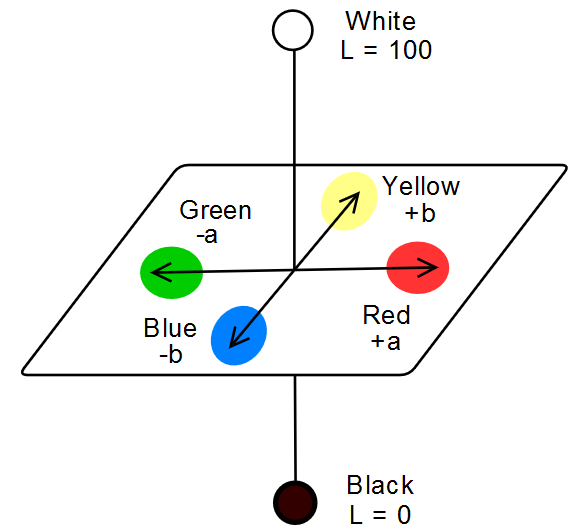
\includegraphics[width=0.4\linewidth]{Imagens/cielab}
	\caption{Representation of the CIE L* a* b* color space.}
	\label{cielab}
\end{figure}

Currently, CIELAB is the most used system for quantitative color description of an object, given its uniformity, ease of acquisition, very low cost and device independence. Considering that this technique facilitates the acquisition of measurements directly on the field, while also avoiding the degradation of the compounds, it becomes an appealing approach in comparison to traditionally used methods such as \gls{hplc} or \gls{uv}. The CIELAB color technique has been applied for instance in the unique identification of skin color for clinical and scientific purposes \citep{weatherall1992skin} and as an optimal color design approach for transforming patients' perception into color elements \citep{liu2014optimal}.

Combining \gls{uv} and CIELAB colorimetric data, the aim of the present case study is to validate a quantification method for carotenoid content estimation in roots of \textit{M. esculenta}, assuming that the statistical and machine learning techniques can correlate these data types, to ultimately detect genotypes of M. esculenta with high contents of carotenoids. Importantly, this study provides tools that can support the plant-breeding program at Epagri (Agricultural Research Company and Rural Extension of the State of Santa Catarina, \href{http://www.epagri.sc.gov.br/}{\nolinkurl{http://www.epagri.sc.gov.br/}}) that aims to obtain genotypes with high levels of pro-vitamin A carotenoids and superior nutritional traits.

\section{Data types}

\subsection{Ultraviolet-visible Data}

Fifty root samples of \textit{M. esculenta} genotypes harvested in 2015/2016 season from the Epagri's germplasm bank were used due to their economic and social importance. Samples were visually selected for high content in carotenoids with provitamin A activity and lycopene. 

After carotenoid extraction from the roots using organosolvents, extracts absorbances were then recorded using a spectral window from 200 to 700 $\eta m$. Aliquots of the extracts were also injected into a liquid chromatograph for carotenoid quantification purposes. 

Considering that most carotenoids exhibit absorption in the visible region of
the spectrum, between 400 to 500 $\eta m$, a subset of the original UV-visible
dataset with samples belonging to this wavelength interval was used. Missing values contained within this dataset were replaced with the mean of the variables' values.

In order to accurately predict the carotenoid contents in cassava roots regression-derived statistical and machine learning models were used, including \gls{pls}, decision trees, \gls{svm}s, random forests and neural networks. Three response variables were used in the machine learning approach: the \gls{tcc} determined by spectrophotometry (Lambert-Beer law), the \gls{tcc} and the content of trans-$\beta$-carotene, the most abundant carotene in cassava roots, both determined by HPLC.

Models that showed best performance were selected and the variable importance calculated. Various pre-processing methods were applied to the datasets to see whether model performance could be improved, using these models. The data was also subject to filter-based feature selection (40\%, 60\% and 80\% data filtering) to determine once again if it could improve model performance.


\subsection{CIELAB Data}

Immediately after harvest, color measurements of the root samples were made. For all fifty samples, three readings were performed at different sites.

The analysis pipeline was similar for the CIELAB dataset, however, models that included feature selection, the data pre-processing and filtering processes were excluded from the analysis pipeline, as it did not make sense to perform these, considering there are only 3 features in the dataset (L* a* and b* parameters), while pre-processing was meant for spectral data.

\subsection{Fusion Data}

For the fusion dataset, which contained 104 variables (absorbance values + L* a* b* parameters), the analysis pipeline was similar to that of the CIELAB dataset, while data filtering was also performed similarly to the \gls{uv} dataset.

\section{Data Overview}

In \autoref{cassava_summary} the summary of the different datasets used throughout this analysis pipeline is shown, giving an overall understanding of the datasets composition. 

\begin{figure}[H]
	\centering
	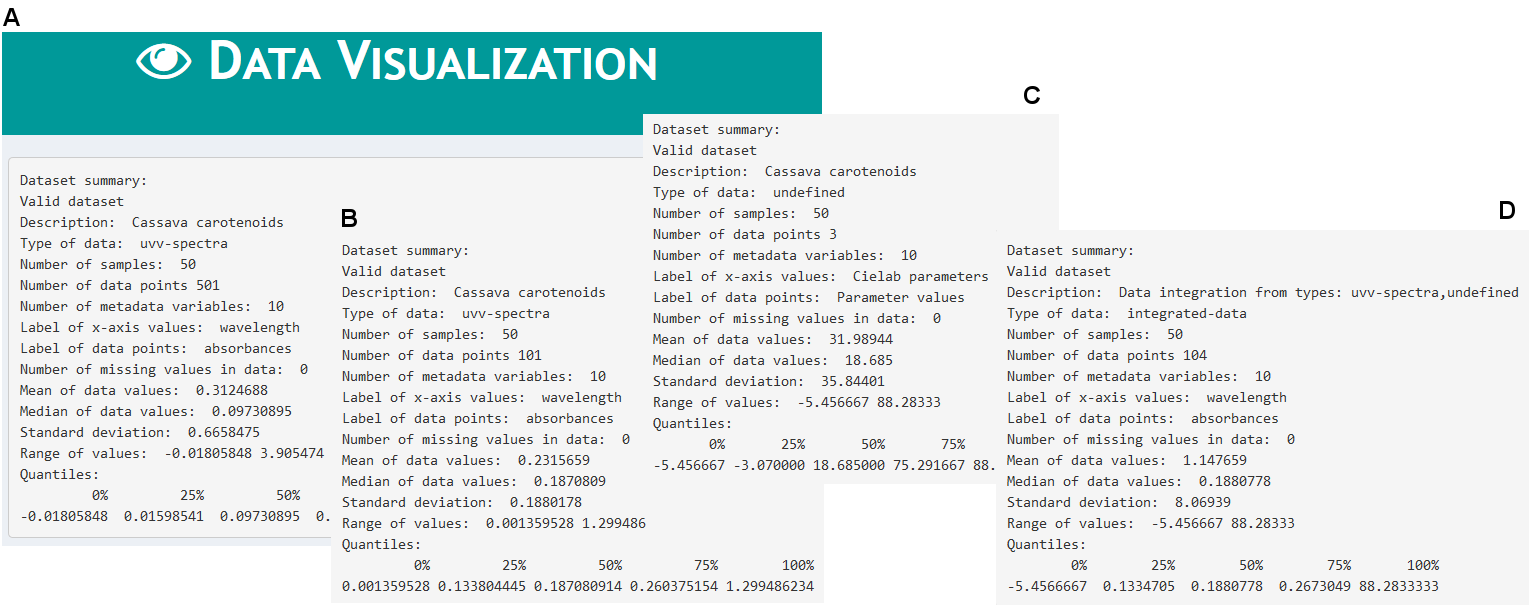
\includegraphics[width=1\linewidth]{Imagens/Case_study/summary_subset_full}
	\caption{Summary of the cassava full \gls{uv} dataset (\textbf{A}) and its subset (wavelengths between 400 and 500 $\eta m$) (\textbf{B}), the CIELAB dataset (\textbf{C}) and the fusion dataset (\textbf{D}).}
	\label{cassava_summary}
\end{figure}

This includes the summary of the cassava full \gls{uv} dataset (\autoref{cassava_summary}A) and its subset with wavelengths between 400 and 500 $\eta m$ (\autoref{cassava_summary}B), the CIELAB dataset (\autoref{cassava_summary}C) and the fusion dataset (\autoref{cassava_summary}D). All datasets are valid, having no missing values they are, therefore, ready for the analysis.

The UV-visible spectrophotometric profiles measured between 200-700 $\eta m$ clearly allow us to discriminate samples according to their carotenoid content. This is more noticeable when comparing the profiles of cassava samples
5, 23 and 74 (\autoref{cassava_spectra_plot}).

\begin{figure}[H]
	\centering
	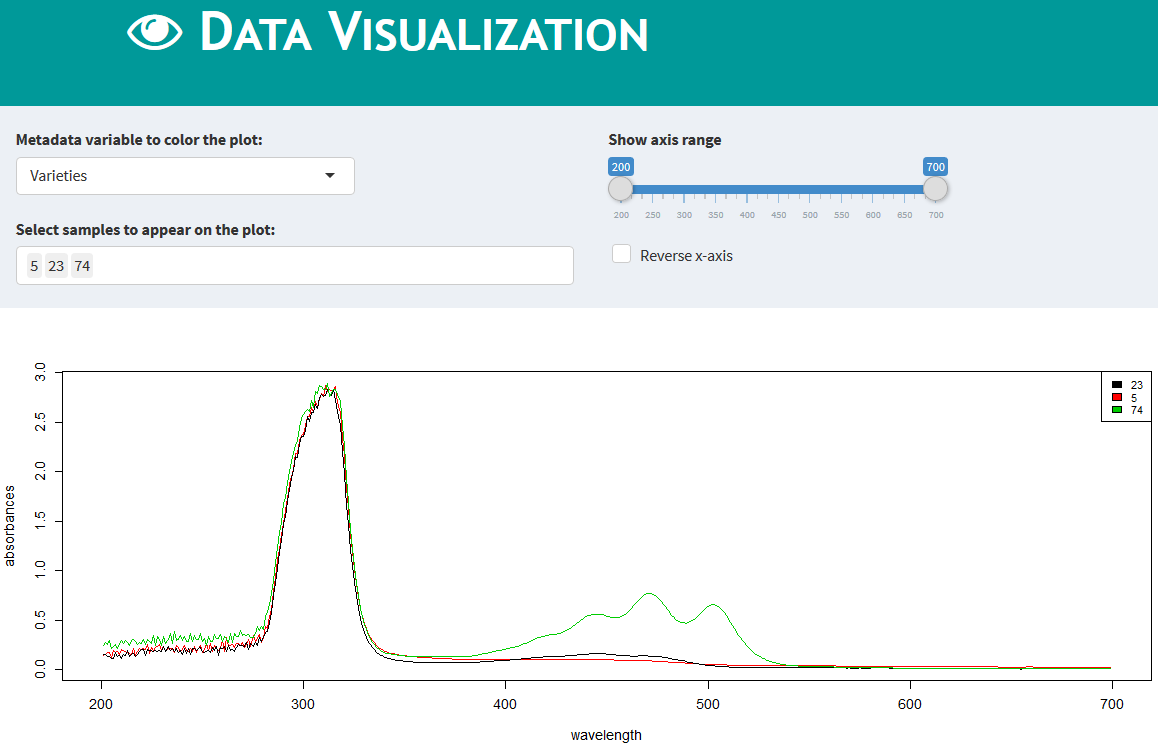
\includegraphics[width=0.8\linewidth]{Imagens/Case_study/spectra_plot}
	\caption{The \gls{uv} spectrophotometric profiles (200 to 700 $\eta m$) of cassava root sample 5 (red), sample 23 (black) and sample 74 (green).}
	\label{cassava_spectra_plot}
\end{figure}

These three samples vary greatly in color, with sample 5 having a cream color, sample 23 a yellow one and the sample 74 a reddish color. The spectrophotometric profiles for these samples differ mostly from each other only at the region of 400-500 $\eta m$, which is precisely the region where carotenoids typically show absorbance peaks. The cream colored sample profile shows an absence of absorbance peaks in this region, while the yellow colored sample shows a small peak. The reddish sample, however, presents three peaks of great absorption in this region of the spectrum. It is, therefore, expected that the more colored the root the higher carotenoid content it possesses.



\section{Univariate Analysis}

To detect significant statistical differences (p-value below 0.05) derived from the effects of cassava's root colors on the spectral profiles a one-way \gls{anova} with Tukey's \gls{hsd} analysis was performed for all wavelengths (200 to 700 $\eta m$). \autoref{cassava_anova}A shows the top ten results ordered by decreasing p-value. In \autoref{cassava_anova}B the -log$_{10}$ of p-values plot is represented, showing an horizontal line that corresponds to a p-value threshold of 0.05. More information about these methods is available in \autoref{univariate}.

From \autoref{cassava_anova} it appears that wavelengths around 500$\eta m$ have a significant effect on the discrimination of cassava samples according to their color. This finding becomes more evident when looking at the -log$_{10}$ of p-values plot.

\begin{figure}[H]
	\centering
	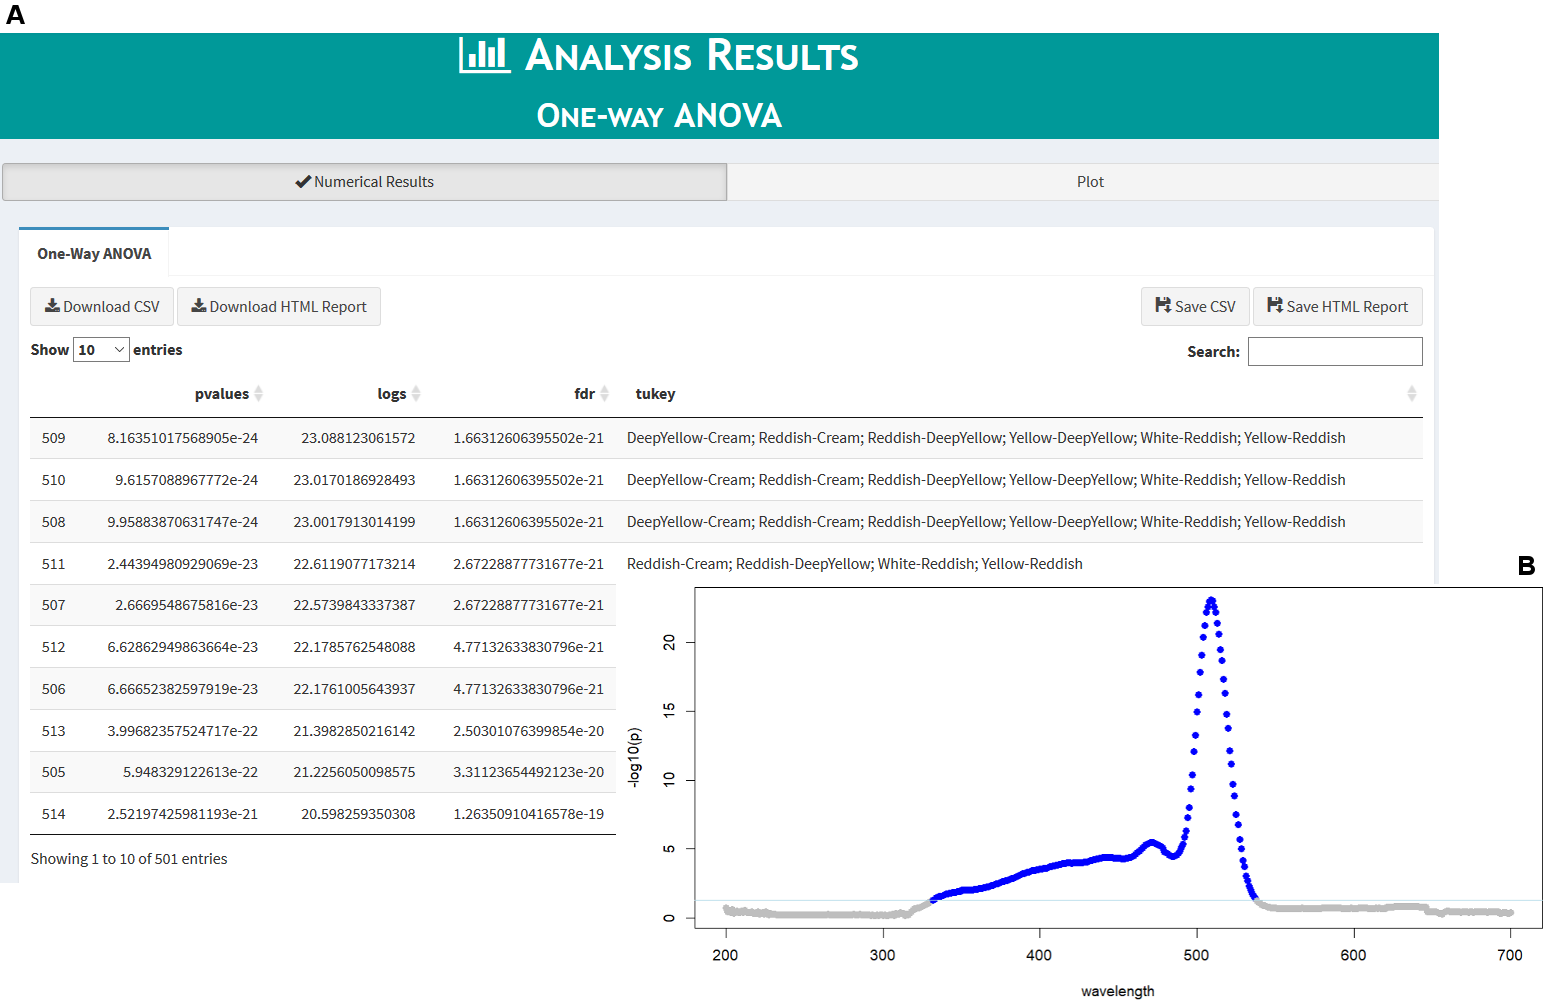
\includegraphics[width=1\linewidth]{Imagens/Case_study/anova_table_plot}
	\caption{\gls{anova} results using the \textit{colors} metadata variable (\textbf{A}) and respective plot of the -log$_{10}$ of p-values with a p-value threshold value of 0.05 (\textbf{B}).}
	\label{cassava_anova}
\end{figure}




\section{Principal Components Analysis}

A \gls{pca} was also performed over the subset \gls{uv} dataset. In their set, PC1 and PC2 explain about 99.5\% of the total variance of the sample population data under this study (\autoref{cassava_pca_scree}). Information regarding this method is available in \autoref{unsupervised}. The performed \gls{pca} resulted in genotype grouping according to the root pulp coloration, as well as carotenoid quantification, with samples 74, 105, 119, and 125 being the most discrepant within this sample universe \autoref{cassava_pca_scores2D}. Interestingly, these are the samples with the highest carotenoid contents among all samples. 

\begin{figure}[H]
	\centering
	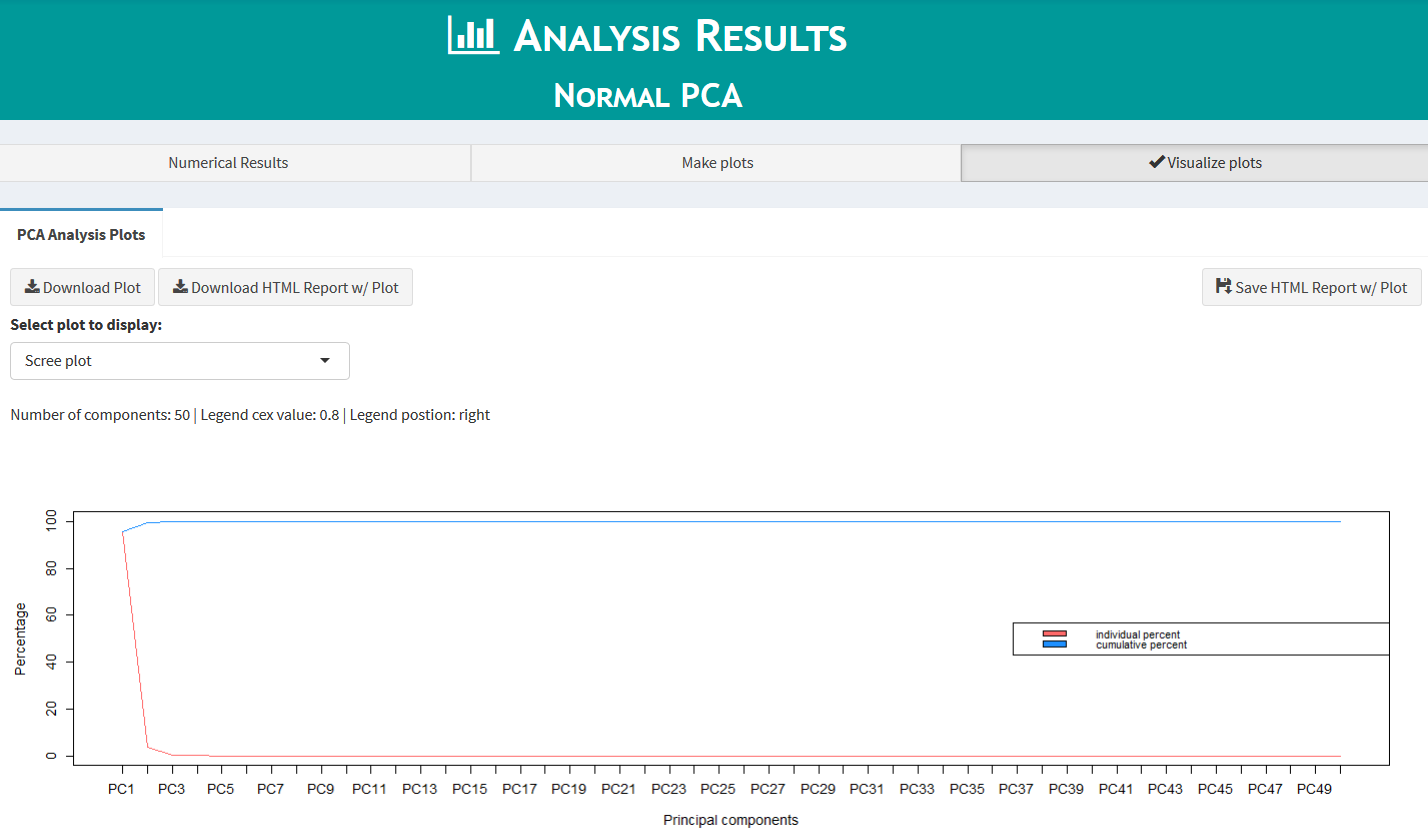
\includegraphics[width=0.8\linewidth]{Imagens/Case_study/pca_scree_plot}
	\caption{Scree plot of the \gls{pca} resulting from the UV-visible spectrophotometric data (400-500 $\eta m$).}
	\label{cassava_pca_scree}
\end{figure}



\begin{figure}[H]
	\centering
	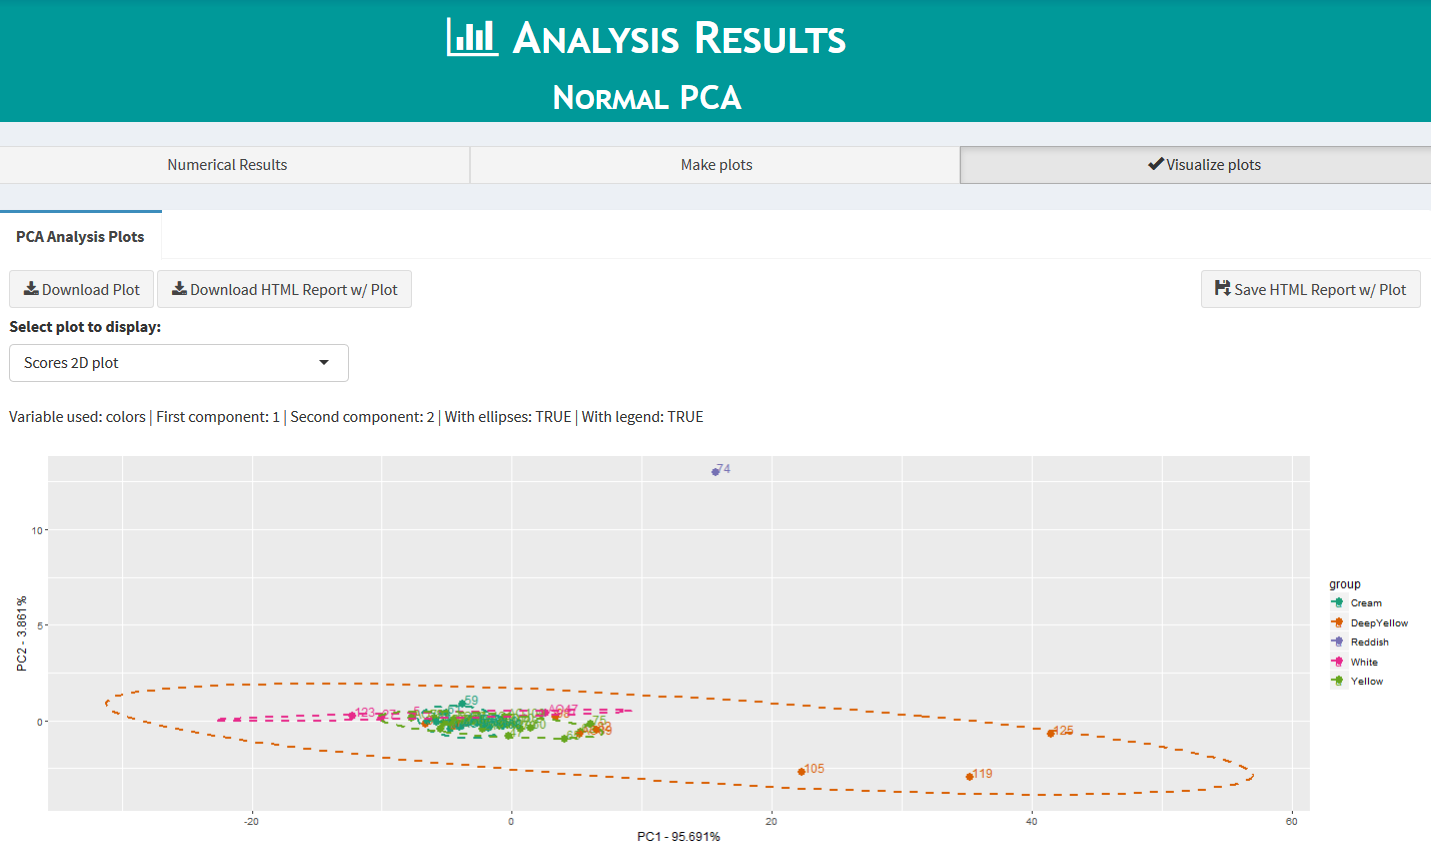
\includegraphics[width=0.8\linewidth]{Imagens/Case_study/pca_scores2Dplot}
	\caption{Scores plot with the distribution of the fifty samples on the first and second \gls{pca} components resulting from the UV-visible spectrophotometric data (400-500 $\eta m$).}
	\label{cassava_pca_scores2D}
\end{figure}


\section{Machine Learning}

In \autoref{cassava_ml} the performance values (RMSE and R$^{2}$) obtained for the different machine learning models trained with UV-visible spectrophotometry data (400-500 $\eta m$), CIELAB data and a \gls{llf} of the two are shown. The response prediction variables used were the \gls{tcc} determined by spectrophotometry (Lambert-Beer formula), the \gls{tcc} determined by HPLC and the total content of trans-$\beta$-carotene (the most abundant carotene in cassava roots). All the results within this section were obtained directly with \textit{specmine}, as the web platform cannot yet approach regression problems. Information regarding this topic is available in \autoref{supervised}.

\begin{table}[H]
	\centering
	\caption{Performance values (RMSE and R$^{2}$) obtained for the different machine learning models trained with UV-visible spectrophotometry data (400-500 $\eta m$), CIELAB data and a \gls{llf} of the two. The \acrfull{tcc} determined by spectrophotometry (Lambert-Beer formula), the \gls{tcc} determined by HPLC and the total content of trans-$\beta$-carotene (the most abundant carotene in cassava roots) were used as response prediction variables.}
	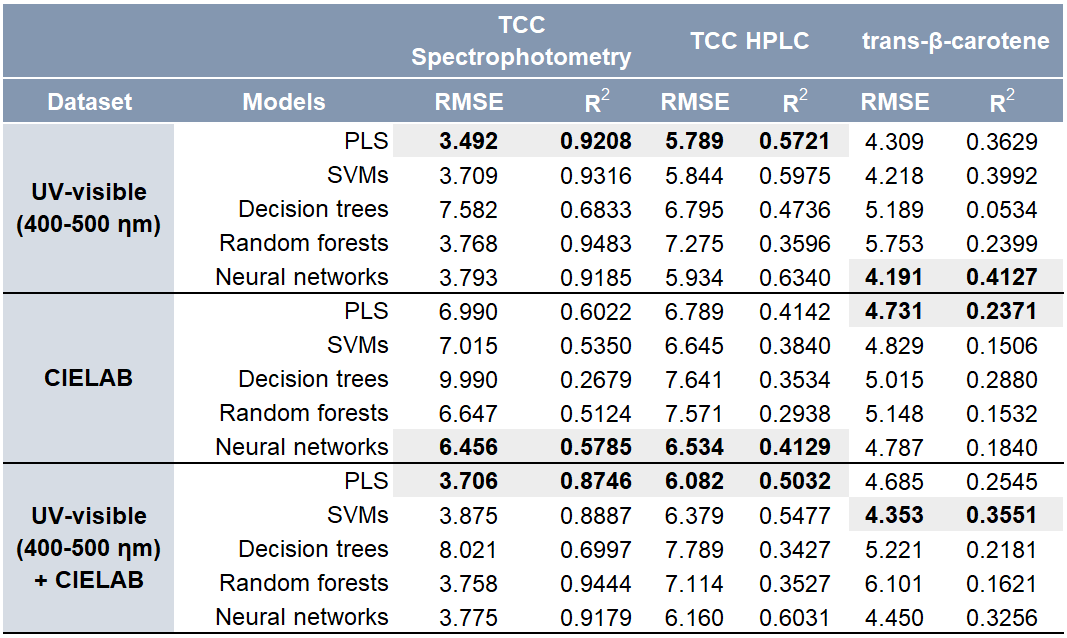
\includegraphics[width=0.9\linewidth]{Imagens/Case_study/ml_table}
	\label{cassava_ml}
\end{table}

Using the \gls{uv} dataset as input, it becomes clear that the highest R$^{2}$ and lowest RMSE performance values were obtained when using the \gls{tcc} determined using spectrophotometric data as response prediction variable. This was somewhat expected considering that both input and response data used employ the same physical phenomenon of detection of compounds (absorbance). 

The \gls{pls} model showed best results for the \gls{tcc} Spectrophotometry and \gls{tcc} HPLC response variables with RMSE and R$^{2}$ values of 3.492, 5.789, 0.92 and 0.57, respectively. For the trans-$\beta$-carotene variable the best model was neural networks with a RMSE of 4.191 and R$^{2}$ of 0.41.

The \gls{vip} values for this case (\autoref{cassava_vips}), which identify the most relevant variables for the validation of the method, show that the wavelengths 449, 448 and 450 $\eta m$ (precisely the wavelength that is used for the quantification of $\beta$-carotene through the Lambert-Beer formula) were used in 100\%, 99.93\% and 99.76\% of cross-validation training performance. This result is important because it attests to the robustness of the models in predicting the contents of these compounds in cassava samples.

\begin{table}[h]
	\centering
	\caption{Top 10 \acrfull{vip} values for the best performing models when using each of the three datasets as input.}
	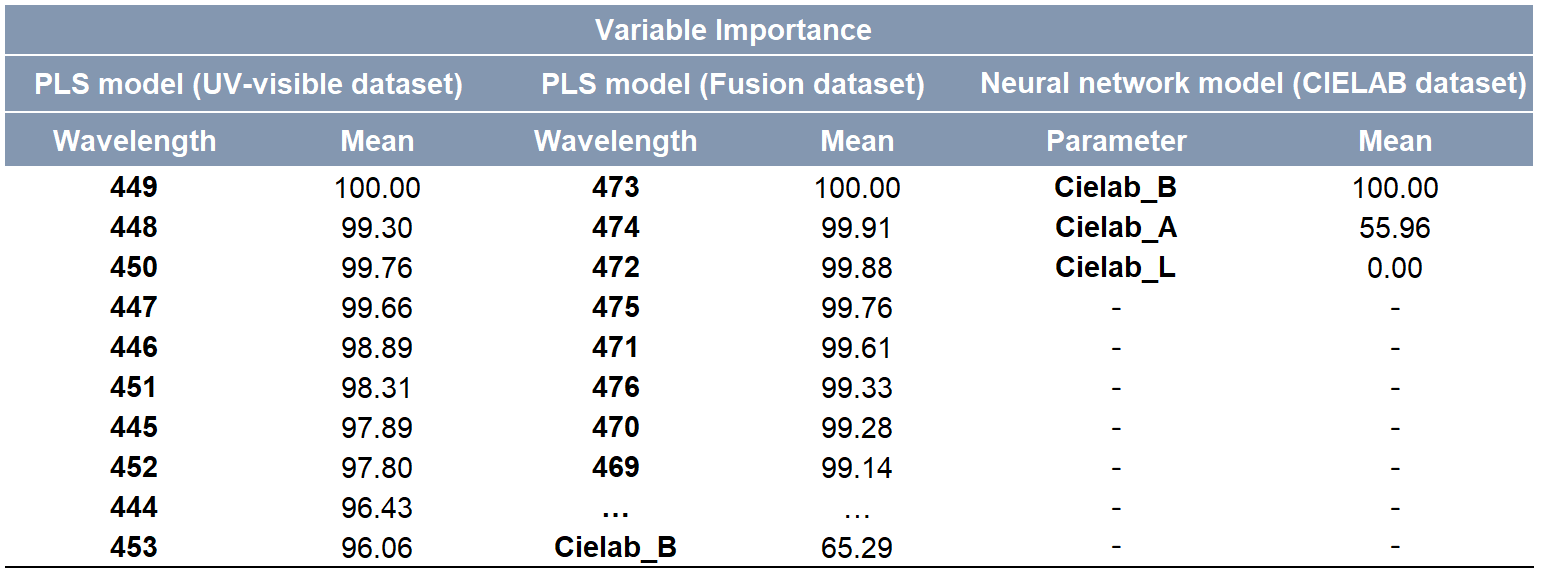
\includegraphics[width=0.9\linewidth]{Imagens/Case_study/ml_vips}
	\label{cassava_vips}
\end{table}


Applying pre-processing methods to the data, as well as feature selection, showed an overall increase in model performance for most models used. one such case is shown in \autoref{cassava_preproc}, where using pre-processed UV-visible data as input to random forest model was able to increase model performance. By applying smoothing interpolation, background and offset corrections, or background correction alone, RMSE values decreased from 6.194 to 5.773, 5.936 and 6.175, respectively. R$^{2}$ values also increased from 55\% to around 60\% in each case.

\begin{table}[h]
	\centering
	\caption{Performance values (RMSE and R$^{2}$) obtained for a random forest model trained with UV-visible spectrophotometry data (400-500 $\eta m$), applying several pre-processing methods to the data. The total carotenoid content (TCC) determined by HPLC was used as response prediction variable.}
	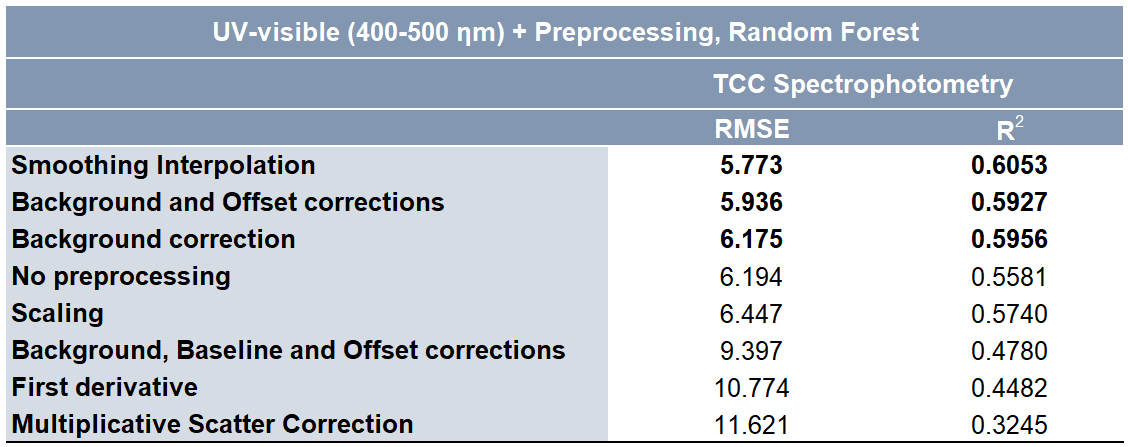
\includegraphics[width=0.9\linewidth]{Imagens/Case_study/ml_preproc}
	\label{cassava_preproc}
\end{table}


When using the CIELAB dataset as input the results obtained were similar to the previous case in the sense that highest R$^{2}$ and lowest RMSE performance values were obtained when using the \gls{tcc} determined using spectrophotometric data as a response prediction variable (\autoref{cassava_ml}). There is, however, a noticeable overall decrease in model performance when using all three prediction variables. This is easily explained by the number of features present in the data, since here only three features are present (L*, a* and b*) whereas in the previous case about 101 features (data measured from 400 to 500 $\eta m$) were present.

The models that showed best performance was neural networks for the \gls{tcc} Spectrophotometry and \gls{tcc} HPLC response variables with RMSE and R$^{2}$ of 6.456, 6.534, 0.58 and 0.41, respectively. \gls{pls} showed best performance using the trans-$\beta$-carotene variable with a RMSE value of 4.731 and R$^{2}$ of 0.23.

Regarding \gls{vip} values for the CIELAB dataset (\autoref{cassava_vips}), it is perceived that the b* parameter was relevant in 100\% of the cases, while the a* parameter was relevant for about 56\% of the predictions, with the L* parameter not being relevant whatsoever with a VIP of 0\%. 

The results obtained using the fusion data were once again similar to the previous cases, considering that highest R$^{2}$ and lowest RMSE performance values were obtained when using the \gls{tcc} Spectrophotometry response variable (\autoref{cassava_ml}). 

The \gls{pls} model showed best results for the \gls{tcc} Spectrophotometry and \gls{tcc} HPLC response variables with RMSE and R$^{2}$ values of 3.706, 6.082, 0.87 and 0.50, respectively. For the trans-$\beta$-carotene variable the best model was \gls{svm}s with a RMSE of 4.353 and R$^{2}$ of 0.35.

The \gls{vip} values computed for this case (\autoref{cassava_vips}) showed that the variables which presented the most important role in the prediction of carotenoid content in the cassava samples were those of wavelength around 170 $\eta m$ (\gls{vip}s $ > $ 99\%). Here, the CIELAB b* parameter was relevant in about 65\% of predictions, while the a* and L* parameters had a VIP close to zero.

These findings altogether have shown how CIELAB color measurement can be used as a fast and non-destructive method to calibrate for the total carotenoid content of cassava genotypes roots with acceptable prediction error. The low-level fusion between \gls{uv} spectrophotometry and CIELAB data has demonstrated how data fusion can lead to a better model performance for prediction when comparing to the use of a single data source, having similar results already been published \citep{botwey2014multi}. Additionally, the \gls{uv} spectrophotometric profiles measured between 400-500 $\eta m$ allowed the observation of a positive correlation between the color of the root pulp and the total carotenoid content, which is in accordance with data reported in the literature \citep{champagne2010carotenoid, chavez2005variation, iglesias1997genetic}.

Reports with more detailed analysis pipelines for each response variable can be found at \href{http://darwin.di.uminho.pt/pacbb2017/cassava-carotenoids/}{\nolinkurl{http://darwin.di.uminho.pt/pacbb2017/cassava-carotenoids/}}.








